%==============================================================================
%  MATH 231 -- Linear Algebra I (Queens College, Fall 2026)
%  SETUP GUIDE 1 -- Git and GitHub
%
%  AUDIENCE: students, many of whom have never used git or a terminal.  Written
%  to be followed top to bottom with nothing assumed.  Keep the reading level
%  low and the checkpoints frequent.
%
%  INSTRUCTOR HANDLE.  The collaborator username is defined ONCE, by the macro
%  \instructorgh below.  Change it there and it updates everywhere.
%
%  NOTE: the course repository lives at github.com/KevinB88/..., so the
%  instructor's account appears to be "KevinB88", but the handle specified for
%  student collaborator invites was "KevBedoya".  If those are the same person
%  with one account, correct \instructorgh before distributing -- an incorrect
%  handle silently blocks every submission.
%
%  Compile with pdflatex (standard TeX Live packages only).
%==============================================================================
\documentclass[11pt]{article}

\usepackage[margin=1in]{geometry}
\usepackage{amsmath,amssymb}
\usepackage[dvipsnames]{xcolor}
\usepackage{enumitem}
\usepackage{booktabs}
\usepackage{array}
\usepackage[hidelinks]{hyperref}
\usepackage{titlesec}
\usepackage{needspace}
\usepackage{listings}
\usepackage{tikz}
\usetikzlibrary{arrows.meta}

%------------------------------------------------------------------ style ----
\titleformat{\section}{\large\bfseries\sffamily\color{RoyalBlue}}
                      {\thesection.}{0.6em}{}
\titleformat{\subsection}{\normalsize\bfseries\sffamily}{\thesubsection.}{0.5em}{}
\titlespacing*{\section}{0pt}{16pt}{7pt}

\lstdefinestyle{term}{
  basicstyle=\ttfamily\small,
  backgroundcolor=\color{gray!10},
  frame=single, rulecolor=\color{gray!45},
  framesep=5pt, xleftmargin=8pt, xrightmargin=8pt,
  breaklines=true, columns=fullflexible, keepspaces=true,
  showstringspaces=false, aboveskip=8pt, belowskip=8pt
}
\lstset{style=term}

\newcommand{\plat}[1]{\smallskip\noindent
  \textcolor{BrickRed}{\sffamily\bfseries #1}\par\nopagebreak\smallskip}
\newcommand{\checkpoint}[1]{\par\smallskip\noindent
  {\small\sffamily\textcolor{ForestGreen}{\textbf{Checkpoint.}}\ #1}\par\smallskip}
\newcommand{\heads}[1]{\par\smallskip\noindent
  {\small\sffamily\textcolor{BrickRed}{\textbf{Watch out.}}\ #1}\par\smallskip}

%------------------------------------------------------------ course facts ---
\newcommand{\instructorgh}{KevBedoya}   % <-- instructor's GitHub username
\newcommand{\repname}{QC\_MATH231}

\title{\vspace{-1.2cm}\textbf{\sffamily MATH 231 -- Linear Algebra I}\\[4pt]
       {\large\sffamily Setup Guide 1 \textbullet\ Git and GitHub}\\[2pt]
       {\normalsize\sffamily Queens College, CUNY \textbullet\ Fall 2026
        \textbullet\ Instructor: Kevin Bedoya}}
\author{}
\date{}

\begin{document}
\maketitle
\vspace{-1.4cm}

\noindent\textbf{What this guide does.} By the end you will have a private
GitHub repository named \texttt{\repname}, a copy of it on your own computer,
three folders inside it for your coursework, and the ability to send your work
to GitHub with two commands. This is how you will hand in every homework,
project, and extra-credit assignment this semester.

\medskip
\noindent\textbf{No experience assumed.} If you have never opened a terminal,
that is fine --- every command you need is written out. Follow the steps in
order. Each one ends with a \textcolor{ForestGreen}{\sffamily\bfseries
Checkpoint} telling you what you should see if it worked. If something goes
wrong, \S\ref{sec:trouble} is a troubleshooting guide covering the problems that
actually happen.

\medskip
\noindent\textbf{Everything here is free.} You will not be asked to pay for
anything or enter a credit card.

%==============================================================================
\section{What git and GitHub are}
%==============================================================================
Two different things with confusingly similar names.

\begin{itemize}[leftmargin=1.4em,itemsep=5pt]
  \item \textbf{git} is a program that runs on \emph{your} computer. It watches
        a folder and records snapshots of it over time. Each snapshot is called
        a \textbf{commit}, and it comes with a short message saying what
        changed. Nothing is ever silently overwritten --- you can always look
        back at what a file used to be.
  \item \textbf{GitHub} is a website that stores copies of those folders online.
        It is where your work goes so that I can see it, and where my feedback
        comes from so that you can see it.
\end{itemize}

\noindent A rough analogy: git is like the version history in Google Docs, and
GitHub is like Google Drive. The important difference is that git only records a
snapshot when you \emph{tell} it to --- it does not autosave.

\begin{center}
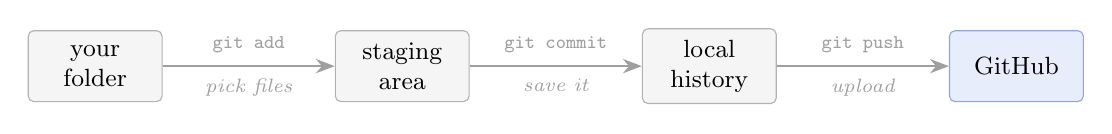
\begin{tikzpicture}[
    box/.style={draw=gray!60, rounded corners=2pt, fill=gray!8, inner sep=4pt,
                font=\small, align=center, minimum height=9mm,
                minimum width=17mm},
    lbl/.style={font=\scriptsize\ttfamily},
    sub/.style={font=\scriptsize\itshape, text=gray!75},
    flow/.style={-{Stealth[length=2.4mm]}, gray!75, thick}]
  \node[box] (a) at (0,0)    {your\\folder};
  \node[box] (b) at (3.9,0)  {staging\\area};
  \node[box] (c) at (7.8,0)  {local\\history};
  \node[box, draw=RoyalBlue!60, fill=RoyalBlue!12] (d) at (11.7,0) {GitHub};
  \draw[flow] (a) -- (b) node[midway,above=1pt,lbl]{git add}
                         node[midway,below=1pt,sub]{pick files};
  \draw[flow] (b) -- (c) node[midway,above=1pt,lbl]{git commit}
                         node[midway,below=1pt,sub]{save it};
  \draw[flow] (c) -- (d) node[midway,above=1pt,lbl]{git push}
                         node[midway,below=1pt,sub]{upload};
\end{tikzpicture}
\end{center}

\noindent That picture is the whole workflow. Sections \ref{sec:folders} and
\ref{sec:workflow} walk through it.

%==============================================================================
\section{Create a GitHub account}
%==============================================================================
Skip this if you already have one.

\begin{enumerate}[leftmargin=2.0em,itemsep=4pt]
  \item Go to \url{https://github.com} and click \textbf{Sign up}.
  \item Enter an email address, a password, and a username. Your username is
        public and hard to change later --- pick something you would not mind me
        or a future employer seeing.
  \item Verify your email address when GitHub sends the confirmation.
\end{enumerate}

\checkpoint{You can sign in at \url{https://github.com} and see your profile
page.}

\heads{Write your username and password down somewhere safe. You will need them
in \S5, and a forgotten password is the single most common reason a student
cannot submit on time.}

%==============================================================================
\section{Create the private repository}
%==============================================================================
A \textbf{repository} --- ``repo'' for short --- is just a folder that git
tracks.

\begin{enumerate}[leftmargin=2.0em,itemsep=5pt]
  \item Sign in to GitHub. Click the \textbf{$+$} in the top-right corner, then
        \textbf{New repository}.
  \item \textbf{Repository name:} type exactly
        \[
          \texttt{\repname}
        \]
        Note the underscore, and that there are no spaces.
  \item \textbf{Description:} optional. Something like ``MATH 231 coursework''
        is fine.
  \item \textbf{Visibility:} choose \textbf{Private}. This matters --- your
        coursework should not be public, both for your privacy and so that
        others cannot copy your solutions.
  \item Under \emph{Initialize this repository with}, tick
        \textbf{Add a README file}. This creates a starting file so the
        repository is not empty, which makes the next steps simpler.
  \item Click \textbf{Create repository}.
\end{enumerate}

\checkpoint{You are looking at a page titled
\texttt{your-username/\repname} with a \emph{Private} label next to the
name, and it contains one file called \texttt{README.md}.}

%==============================================================================
\section{Install git}
%==============================================================================
You need the git program on your own computer. Find your operating system below.

\plat{Windows}
The easiest route is the official installer.

\begin{enumerate}[leftmargin=2.0em,itemsep=3pt]
  \item Go to \url{https://git-scm.com/download/win} and let the download start.
  \item Run the installer. \textbf{Accept every default} by clicking
        \emph{Next} through all the screens --- the defaults are correct and the
        options are not worth reading on a first install.
  \item When it finishes, open the \textbf{Start} menu, type
        \texttt{Git Bash}, and open it. This is a terminal window; you will type
        your git commands here for the rest of the semester.
\end{enumerate}

\noindent If you prefer, you can install from a terminal instead:

\begin{lstlisting}
winget install --id Git.Git -e --source winget
\end{lstlisting}

\plat{macOS}
Open the \textbf{Terminal} app (press \texttt{Cmd}+\texttt{Space}, type
\texttt{Terminal}, press Enter) and run:

\begin{lstlisting}
git --version
\end{lstlisting}

\noindent If git is missing, macOS will pop up a window offering to install the
Command Line Developer Tools. Click \textbf{Install} and wait. If no window
appears, run this instead:

\begin{lstlisting}
xcode-select --install
\end{lstlisting}

\plat{Linux}
Open a terminal and run the line for your distribution:

\begin{lstlisting}
sudo apt update && sudo apt install git      # Ubuntu, Debian, Mint
sudo dnf install git                         # Fedora
sudo pacman -S git                           # Arch
\end{lstlisting}

\subsection*{Check that it worked}
In your terminal (Git Bash on Windows), run:

\begin{lstlisting}
git --version
\end{lstlisting}

\checkpoint{You see something like \texttt{git version 2.43.0}. The exact
number does not matter.}

\subsection*{Tell git who you are}
Git stamps your name and email onto every commit. Set them once, now, or your
first commit will fail with a complaint. Run both lines, substituting your own
details:

\begin{lstlisting}
git config --global user.name "Your Name"
git config --global user.email "your.email@example.com"
\end{lstlisting}

\heads{Use the \emph{same} email address you signed up to GitHub with.
Otherwise your commits will not be linked to your account.}

%==============================================================================
\section{Clone the repository}
%==============================================================================
\textbf{Cloning} means downloading a copy of the GitHub repository onto your
computer, already set up so git knows where it came from.

\begin{enumerate}[leftmargin=2.0em,itemsep=5pt]
  \item On your repository page on GitHub, click the green \textbf{Code} button.
  \item Make sure the \textbf{HTTPS} tab is selected, then click the copy icon
        to copy the address. It looks like
        \texttt{https://github.com/your-username/\repname.git}
  \item In your terminal, move to wherever you want the folder to live. For
        example, to put it on your Desktop:
\begin{lstlisting}
cd Desktop
\end{lstlisting}
  \item Clone it, pasting the address you copied:
\begin{lstlisting}
git clone https://github.com/your-username/QC_MATH231.git
\end{lstlisting}
  \item Move into the new folder:
\begin{lstlisting}
cd QC_MATH231
\end{lstlisting}
\end{enumerate}

\checkpoint{Running \texttt{ls} (or \texttt{dir} on Windows outside Git Bash)
shows \texttt{README.md}. Running \texttt{git status} says
\emph{``On branch main, nothing to commit, working tree clean.''}}

\heads{If git asks for a \textbf{password}, do not type your GitHub password ---
GitHub stopped accepting those in 2021. You need a \emph{personal access token}
instead. \S\ref{ts:token} explains how to make one; it takes about a minute.}

%==============================================================================
\section{Create your folders}\label{sec:folders}
%==============================================================================
Inside the repository, make the three folders where your work will go. From
inside \texttt{\repname}, run:

\begin{lstlisting}
mkdir homework projects extra-credit
\end{lstlisting}

\noindent Now a quirk that catches everybody: \textbf{git tracks files, not
folders.} An empty folder is invisible to git and will never appear on GitHub.
The standard fix is to put one placeholder file in each. On Git Bash, macOS, or
Linux:

\begin{lstlisting}
touch homework/.gitkeep projects/.gitkeep extra-credit/.gitkeep
\end{lstlisting}

\noindent The name \texttt{.gitkeep} has no special meaning to git --- it is
just a conventional name for ``this file exists only so the folder does''. Once
you put real assignments in these folders you can leave the placeholders or
delete them; it makes no difference.

\checkpoint{Running \texttt{git status} now lists \texttt{extra-credit/},
\texttt{homework/} and \texttt{projects/} under \emph{Untracked files}.}

%==============================================================================
\section{Save your work and send it to GitHub}\label{sec:workflow}
%==============================================================================
This is the loop you will repeat all semester. Four commands, in order.

\subsection{See what changed --- \texttt{git status}}
\begin{lstlisting}
git status
\end{lstlisting}

\noindent This changes nothing; it only reports. It tells you which files you
have edited, created, or deleted. Run it whenever you are unsure what state you
are in --- it is the safest command in git.

\subsection{Choose what to save --- \texttt{git add}}
\begin{lstlisting}
git add .
\end{lstlisting}

\noindent The dot means ``everything in this folder''. This does not save
anything yet; it marks files as \emph{ready} to be saved. (You can also name one
file, as in \texttt{git add homework/hw1.py}, but the dot is fine for this
course.)

\subsection{Save the snapshot --- \texttt{git commit}}
\begin{lstlisting}
git commit -m "Add coursework folders"
\end{lstlisting}

\noindent The \texttt{-m} flag supplies the \textbf{message}, in quotes: a short
description of what you did. The message is required. Write something a human
could read later --- \texttt{"Finish homework 1"} is useful,
\texttt{"stuff"} is not.

\checkpoint{Git prints a summary like
\texttt{[main a1b2c3d] Add coursework folders} followed by a count of files
changed.}

\subsection{Upload it --- \texttt{git push}}
\begin{lstlisting}
git push
\end{lstlisting}

\noindent This sends your commits to GitHub. Until you push, your work exists
only on your own computer --- and only pushed work can be graded.

\checkpoint{Refresh your repository page on GitHub in a browser. You now see the
\texttt{homework}, \texttt{projects} and \texttt{extra-credit} folders, and your
commit message next to them.}

\begin{center}
\renewcommand{\arraystretch}{1.4}
\begin{tabular}{@{}l l@{}}
\toprule
\textbf{Command} & \textbf{What it does} \\
\midrule
\texttt{git status}              & shows what has changed; changes nothing \\
\texttt{git add .}               & marks all changes to be saved \\
\texttt{git commit -m "message"} & saves a snapshot, with a description \\
\texttt{git push}                & uploads your saved snapshots to GitHub \\
\texttt{git pull origin main}    & downloads changes from GitHub
                                   (\S\ref{sec:pull}) \\
\bottomrule
\end{tabular}
\end{center}

\noindent Those five are all you need. Git has hundreds of other commands and
you can ignore every one of them for this course.

%==============================================================================
\section{Add me as a collaborator}
%==============================================================================
Your repository is private, so by default nobody but you can see it --- me
included. Adding me as a \textbf{collaborator} lets me read your submissions,
grade them, and push written feedback back into your repository.

\begin{enumerate}[leftmargin=2.0em,itemsep=4pt]
  \item On your repository page, click \textbf{Settings} (in the row of tabs
        near the top, on the right).
  \item In the left sidebar, click \textbf{Collaborators}. GitHub may ask you to
        confirm your password.
  \item Click \textbf{Add people}.
  \item Type my username exactly:
        \[
          \texttt{\instructorgh}
        \]
  \item Select me from the results and click \textbf{Add \instructorgh\ to this
        repository}.
\end{enumerate}

\checkpoint{Under \emph{Manage access} you see my username listed as
\emph{Pending invite}, which becomes \emph{Collaborator} once I accept.}

\heads{Do this \emph{before} the first assignment is due. If I am not a
collaborator I cannot see your work at all, and a submission I cannot see is a
submission that cannot be graded.}

%==============================================================================
\section{Getting my feedback --- \texttt{git pull}}\label{sec:pull}
%==============================================================================
When I grade your work I will push comments and corrections directly into your
repository. Those changes exist on GitHub but not yet on your computer. To bring
them down, run this from inside your \texttt{\repname} folder:

\begin{lstlisting}
git pull origin main
\end{lstlisting}

\noindent Read it as: \emph{pull from the remote called \texttt{origin} (which
is GitHub) the branch called \texttt{main}}. Git downloads whatever is new and
merges it into your local copy.

\medskip
\noindent Make a habit of running \texttt{git pull origin main} \textbf{before}
you start working, not after. If you and I have both changed things, pulling
first keeps them separate and avoids the conflict described in
\S\ref{ts:conflict}.

\checkpoint{Git either reports \texttt{Already up to date.} or lists the files
it just downloaded.}

%==============================================================================
\section{Troubleshooting}\label{sec:trouble}
%==============================================================================
These are the problems that actually come up. Find your error message.

\subsection{``git'' is not recognised / command not found}
\begin{lstlisting}
'git' is not recognized as an internal or external command
bash: git: command not found
\end{lstlisting}
Git either is not installed, or your terminal was open before you installed it
and has not noticed. \textbf{Close the terminal completely and open a new one},
then try \texttt{git --version} again. If it still fails, redo \S4. On Windows,
make sure you are using \textbf{Git Bash} and not Command Prompt.

\subsection{It asks for a password and rejects the right one}\label{ts:token}
GitHub no longer accepts your account password from the command line. You need a
\textbf{personal access token}, which is a long password generated for one
purpose.

\begin{enumerate}[leftmargin=2.0em,itemsep=3pt]
  \item On GitHub, click your profile picture (top right) $\to$
        \textbf{Settings}.
  \item Scroll to the very bottom of the left sidebar $\to$
        \textbf{Developer settings}.
  \item \textbf{Personal access tokens} $\to$ \textbf{Tokens (classic)} $\to$
        \textbf{Generate new token (classic)}.
  \item Give it a note like \texttt{MATH 231}, set an expiry (a year is fine),
        and tick the \textbf{repo} checkbox.
  \item Click \textbf{Generate token}, then \textbf{copy it immediately} ---
        GitHub will never show it to you again.
  \item When git asks for a password, paste the token instead.
\end{enumerate}

\noindent Store the token somewhere safe, like a password manager or a note on
your phone.

\subsection{``Please tell me who you are''}
\begin{lstlisting}
*** Please tell me who you are.
\end{lstlisting}
You skipped the configuration at the end of \S4. Run the two
\texttt{git config --global} lines and commit again.

\subsection{My folder does not appear on GitHub}
It is empty, and git does not track empty folders. Put a file in it --- see the
\texttt{.gitkeep} step in \S\ref{sec:folders} --- then \texttt{add},
\texttt{commit}, and \texttt{push} again.

\subsection{``fatal: not a git repository''}
You are running a git command from the wrong place. Git commands only work
inside a cloned repository. Run:

\begin{lstlisting}
cd QC_MATH231
\end{lstlisting}

\noindent and try again. Use \texttt{pwd} to see which folder you are currently
in.

\subsection{``nothing to commit, working tree clean''}
Git sees no changes. Usually this means you forgot to \emph{save} the file in
your editor, or you already committed the change. Check with
\texttt{git status}.

\subsection{``Updates were rejected''}
\begin{lstlisting}
! [rejected]  main -> main (fetch first)
\end{lstlisting}
GitHub has commits that your computer does not --- typically feedback I pushed.
Download them first, then push again:

\begin{lstlisting}
git pull origin main
git push
\end{lstlisting}

\subsection{It opened a strange full-screen text editor}
You ran \texttt{git commit} without \texttt{-m}, so git opened an editor to ask
for the message. If it looks like a plain screen with tildes down the left, that
is Vim: press \texttt{Esc}, then type \texttt{:q!} and press Enter to escape.
Then commit properly with the message on the command line:

\begin{lstlisting}
git commit -m "your message here"
\end{lstlisting}

\subsection{Merge conflict}\label{ts:conflict}
If a pull reports a \emph{conflict}, it means the same lines were changed in two
places and git cannot decide which to keep. Do not guess and do not delete the
folder. Take a screenshot of the message and contact me --- these are quick to
fix when someone talks you through them, and this course will rarely produce
one.

\subsection{Still stuck}
Email me at \url{Kevin.Bedoya32@stu-mail.qc.cuny.edu} or ask on the class
Discord. Include:

\begin{itemize}[leftmargin=1.4em,itemsep=2pt,topsep=3pt]
  \item your operating system,
  \item the exact command you typed, and
  \item the full error message, copied as text or as a screenshot.
\end{itemize}

\noindent Nobody is expected to arrive knowing this. Ask early --- a setup
problem the night before a deadline is a setup problem solved too late.

\end{document}
